\documentclass[../main.tex]{subfile}
\graphicspath{{\subfix{../images}}}
\begin{document}

这项工作中使用的卷积神经网络需要$227\times 227$像素的固定输入尺寸。对于检测,我们考虑的物体候选是任意的矩形图像。我们评估了两种将物体候选转化为有效的CNN输入的方法。

第一种方法("带上下文的最紧密正方形")将每个物体候选包围在最紧密正方形内,然后将该正方形所包含的图像(各向同性)缩放到CNN输入尺寸。图\ref{fig:transformations}(B)列显示了这种转换。这种方法的一个变种("无上下文的最紧密正方形")排除了围绕原始物体候选的图像内容。图\ref{fig:transformations}(C)列显示了这种转换。第二种方法("扭曲")以各向异性的方式将每个物体候选扩展到CNN的输入尺寸。图\ref{fig:transformations}(D)列显示了扭曲的变换。

\begin{figure}[H]
    \centering
    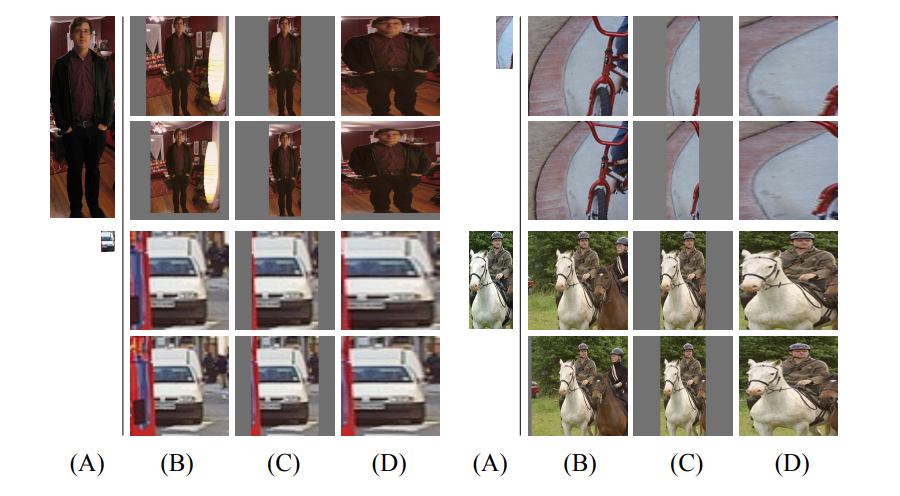
\includegraphics[width=\textwidth]{transformations.png}
    \caption{\textbf{不同的物体候选转换。}(A)相对于转换后的CNN输入的实际比例的原始物体候选;(B)带上下文的最紧密正方形;(C)无上下文的最紧密正方形;(D)扭曲。在每一列和例子的候选中,最上面一行对应的是$p=0$像素的上下文填充,而最下面一行则是$p=16$像素的上下文填充。}
    \label{fig:transformations}
\end{figure}

对于每一个转换,我们也考虑在原始物体候选周围包括额外的图像背景。上下文填充量($p$)被定义为转换后的输入坐标帧中原始对象建议周围的边界大小。图\ref{fig:transformations}顶部展示了每个例子中$p=0$像素的情况,底部展示了$p=16$像素的情况。在所有的方法中,如果源矩形超出了图像,缺失的数据将被替换为图像的平均值(然后在将图像输入到CNN之前将其减去)。一组试验表明,带有上下文填充的扭曲($p=16$像素)在很大程度上胜过了其他方法(3-5个mAP点)。显然,更多的替代方案是可能的,包括使用复制而不是平均填充。对这些替代方案的详尽评估将作为未来的工作。

\end{document}